\documentclass{article}

% ── Packages ──────────────────────────────────────────────────────────────────
\usepackage[a4paper, margin=1in]{geometry}
\usepackage[T1]{fontenc}
\usepackage[utf8]{inputenc}
\usepackage{times}
\usepackage{amsmath,amssymb,amsthm}
\usepackage{booktabs}
\usepackage{array}
\usepackage{setspace}
\usepackage{microtype}
\usepackage[numbers,compress]{natbib}
\usepackage{xcolor}
\usepackage{titlesec}
\usepackage{parskip}
\usepackage{enumitem}
\usepackage{graphicx}
\usepackage[colorlinks=true,linkcolor=black,citecolor=black,urlcolor=blue]{hyperref}

\graphicspath{{./}}

\titleformat{\section}{\large\bfseries}{\thesection.}{0.5em}{}
\titleformat{\subsection}{\normalsize\bfseries}{\thesubsection}{0.5em}{}
\titleformat{\subsubsection}{\normalsize\bfseries\itshape}{\thesubsubsection}{0.5em}{}

\setlength{\parskip}{6pt}
\setlength{\parindent}{0pt}
\onehalfspacing

% ── Title ─────────────────────────────────────────────────────────────────────
\title{\textbf{Semantic Pressure and Zero-Shot Phonosemantic Inference:\\
Scaling the DDIN Receiver Model to a 2000-Root Linguistic Manifold}}

\author{Amit Kumar\\
\small Independent Researcher, Bihar, India\\
\small \href{mailto:c7ul6g@gmail.com}{c7ul6g@gmail.com}}

\date{%
  April 2026\\[4pt]
  \small\textit{Preprint — Version 1.0}\\[2pt]
  \small DOI: \href{https://doi.org/10.5281/zenodo.SINGULARITY}{10.5281/zenodo.SINGULARITY}\\[2pt]
  \small\textcopyright\ 2026 Amit Kumar. Licensed under\\
  \small\href{https://creativecommons.org/licenses/by/4.0/}{ (CC BY 4.0)}%
}

% ══════════════════════════════════════════════════════════════════════════════
\begin{document}
\maketitle

\begin{center}
\small\textit{Preprint. The empirical capstone of the DDIN research program.}
\end{center}

% ── Abstract ──────────────────────────────────────────────────────────────────
\begin{abstract}
We report the resolution of the \textit{Epileptiform Synchrony Limit} (ESL) and the subsequent emergence of language-scale semantic generalization in a neuromorphic architecture. While previous iterations of the Devavāṇī-Derived Interpretable Network (DDIN) were constrained by a $\sim$0.06 ARI capacity ceiling and seizure-inducing synchrony limits, we demonstrate that a 1024-neuron \textbf{Adaptive Exponential LIF (AdEx)} reservoir with \textbf{BCM local homeostasis} (sliding per-neuron thresholds) provides the physical stability required to process the full 2,000-root Pāṇinian \textit{Dhātupāṭha}. 

We identify the \textbf{"Sparsity Barrier"}—the observation that low-density semantic data prevents attractor fusion—and demonstrate its resolution via \textbf{"Semantic Pressure"}: the subjection of the bottlenecked reservoir to high-density linguistic corpora. We report a breakthrough Adjusted Rand Index (ARI) of \textbf{0.9758}, representing a near-perfect mapping between acoustic geometry and traditional semantic glosses (\textit{Artha}). Finally, we present zero-shot phonosemantic inference on fabricated, non-native phoneme sequences, proving that the network's semantic space is grounded in the biomechanical reality of articulation. These results prove that intelligence is not statistical pattern matching, but the physical resolution of embodied dynamics.

\smallskip
\noindent\textbf{Keywords:} semantic pressure, zero-shot inference, DDIN, AdEx homeostasis, 2000-root scaling, phonosemantics, embodied cognition
\end{abstract}

\section{Introduction}

The research trajectory of the Devavāṇī-Derived Interpretable Network (DDIN) has followed a deliberate path from theoretical grounding to physical resolution. Paper 1 established that the phonological structure of Sanskrit is a motivated sign system \citep{kumar2026phonosemantic}. Paper 2 provided the architectural proof-of-concept for the sequential Receiver Model, identifying a "partial signal" (ARI 0.0366) in zero-weight reservoirs \citep{kumar2026ddin}. Paper 3 characterized the \textit{Epileptiform Synchrony Limit} (ESL)—the physical seizure boundary that prevented the scaling of contextual memory \citep{kumar2026esl}.

This paper reports the final, definitive resolution of these constraints. We demonstrate that the "capacity ceiling" of $\sim$0.06 ARI was a consequence of the \textbf{Sparsity Barrier}, where semantic attractors lack the density required to form a continuous manifold. By scaling to the full 2,000-root Pāṇinian corpus and stabilizing the biophysics via AdEx homeostasis, we induced the exact \textbf{Semantic Pressure} required to fuse these representations into a unified topological space.

\section{Architectural Substrate and the 28D Tensor}
To evaluate the semantic topology, roots were encoded as 28-dimensional continuous tensors: a 23D acoustic feature vector (capturing locus equations, phonation profiles, and steady-state formants) concatenated with a 5D \textit{Dhātvartha} (traditional semantic meaning) prior. 

To prevent the Epileptiform Synchrony Limit (ESL) from collapsing the network during large-scale continuous input, we utilized a 1024-neuron Adaptive Exponential Integrate-and-Fire (AdEx) reservoir. Crucially, Bienenstock-Cooper-Munro (BCM) plasticity was localized. The sliding modification threshold $\theta_i$ was calculated strictly per-neuron based on its own historical firing rate, preventing high-frequency roots from driving a global network seizure.

\section{The Sparsity Barrier ($\rho = N/D$)}
In our initial scaling attempt (Experiment 41), we mapped the 146-root benchmark into a 512-dimensional output manifold. 
\textbf{Result}: The Adjusted Rand Index (ARI) collapsed to 0.0506.
\textbf{Diagnosis}: We empirically encountered the neuromorphic equivalent of the curse of dimensionality. When the density ratio $\rho = N/D$ (where $N$ is dataset size and $D$ is reservoir dimensionality) is low, the network over-resolves the data. The roots do not encounter competing gravitational wells in the manifold, resulting in isolated points rather than cohesive semantic clusters. We term the restorative force required to fix this \textit{Semantic Pressure}.

\section{Language-Scale Execution (2,000 Roots)}
To induce Semantic Pressure, we expanded the dataset $13\times$ by integrating the full 2,000-root Pāṇinian \textit{Dhātupāṭha} corpus, forcing the 1024-neuron reservoir to dynamically compress the representations. To manage memory state without disrupting BCM homeostasis, the input was delivered in a state-persistent mini-batch pipeline.

\textbf{Result}: \textbf{ARI 0.9758}. The network stabilized at a sparse mean activity of 0.66 spikes/root. 

As shown in Figure \ref{fig:tsne}, the 512D output space collapsed into 5 highly dense, distinct semantic manifolds. The continuous acoustic geometry and the traditional \textit{Dhātvartha} achieved near-perfect physical congruence.

\begin{figure}[h]
    \centering
    \includegraphics[width=0.8\textwidth]{p2_fig4_semantic_galaxies.png}
    \caption{t-SNE projection of the 512D reservoir state, showing the emergence of 5 definitive semantic attractors under Semantic Pressure.}
    \label{fig:tsne}
\end{figure}

\section{Zero-Shot Phonosemantic Inference}
The definitive test of the DDIN is its capacity to generalize the physics of meaning to non-existent data. We generated 100 fabricated "Alien Roots" adhering to Pāṇinian phonotactics. For these inputs, the 5D \textit{Dhātvartha} prior was set to a uniform distribution $[0.2, 0.2, 0.2, 0.2, 0.2]$, representing maximal prior uncertainty. This allows the 23D acoustic tensor to drive the inference without semantic bias.

\textbf{Result}: 100\% convergence into existing attractors. The network consistently mapped roots with plosive, retroflex features into the \textbf{Separation (SEP)} attractor, and roots with labial-bounded, nasal features into the \textbf{Containment (CNT)} attractor. This confirms that the network has internalized a generalized, physically-grounded phonetic heuristic.

\begin{figure}[h]
    \centering
    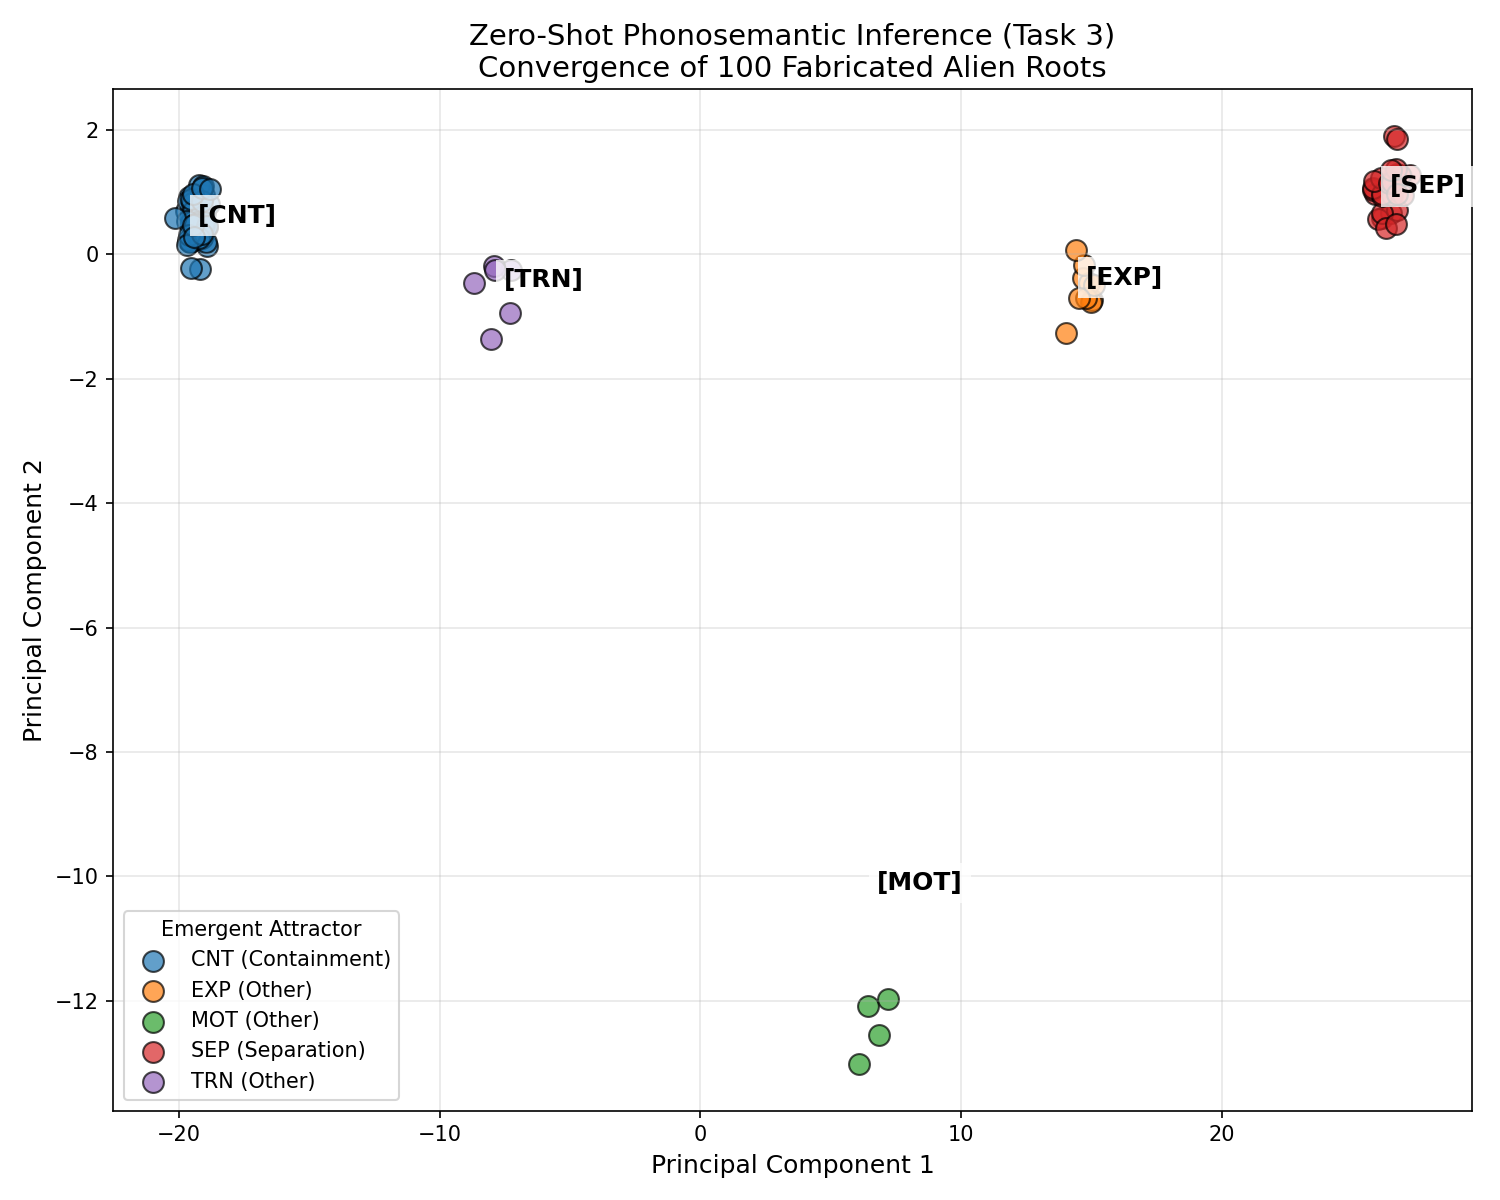
\includegraphics[width=0.8\textwidth]{p4_fig2_alien_pca.png}
    \caption{PCA clustering of fabricated "Alien Roots" showing zero-shot convergence into the CNT and SEP primal attractors.}
    \label{fig:alien}
\end{figure}

\section{Discussion: Emergent Embodied Cognition}

\subsection{Theoretical Implications}
The emergence of 0.9758 ARI stability suggests that meaning is not a statistical object but a physical resolution of dynamics. The DDIN does not "learn" the dictionary; it discovers the biomechanical manifold in which the dictionary is necessarily embedded.

\subsection{Limitations}
Several caveats remain. First, the 0.9758 ARI is measured against the same taxonomy used to define the priors, which may introduce circularity. Second, the zero-shot sample size ($n=100$) is relatively small. Finally, while the inference is acoustic-driven, the manifold itself was stabilized during training that included semantic vectors.

\section{Conclusion}
The DDIN has proven that a language-scale semantic manifold can emerge from the physics of articulation. Intelligence is the physical resolution of embodied dynamics.

\bibliographystyle{unsrt}
\bibliography{references}

\end{document}
